%%%%%%%%%%%%%%%%%%%%%%%%%%%%%%%%%%%%%%%%
% Arsclassica Article
% LaTeX Template
% Version 1.1 (10/6/14)
%
% This template has been downloaded from:
% http://www.LaTeXTemplates.com
%
% Original author:
% Lorenzo Pantieri (http://www.lorenzopantieri.net) with extensive modifications by:
% Vel (vel@latextemplates.com)
%
% License:
% CC BY-NC-SA 3.0 (http://creativecommons.org/licenses/by-nc-sa/3.0/)
%
%%%%%%%%%%%%%%%%%%%%%%%%%%%%%%%%%%%%%%%%%

%----------------------------------------------------------------------------------------
%	PACKAGES AND OTHER DOCUMENT CONFIGURATIONS
%----------------------------------------------------------------------------------------

\documentclass[
11pt, % Main document font size
a4paper, % Paper type, use 'letterpaper' for US Letter paper
oneside, % One page layout (no page indentation)
%twoside, % Two page layout (page indentation for binding and different headers)
headinclude,footinclude, % Extra spacing for the header and footer
BCOR5mm, % Binding correction
]{scrartcl}
%%%%%%%%%%%%%%%%%%%%%%%%%%%%%%%%%%%%%%%%%
% Arsclassica Article
% Structure Specification File
%
% This file has been downloaded from:
% http://www.LaTeXTemplates.com
%
% Original author:
% Lorenzo Pantieri (http://www.lorenzopantieri.net) with extensive modifications by:
% Vel (vel@latextemplates.com)
%
% License:
% CC BY-NC-SA 3.0 (http://creativecommons.org/licenses/by-nc-sa/3.0/)
%
%%%%%%%%%%%%%%%%%%%%%%%%%%%%%%%%%%%%%%%%%

%----------------------------------------------------------------------------------------
%	REQUIRED PACKAGES
%----------------------------------------------------------------------------------------

\usepackage[
nochapters, % Turn off chapters since this is an article        
beramono, % Use the Bera Mono font for monospaced text (\texttt)
%eulermath,% Use the Euler font for mathematics
pdfspacing, % Makes use of pdftex’ letter spacing capabilities via the microtype package
dottedtoc % Dotted lines leading to the page numbers in the table of contents
]{classicthesis} % The layout is based on the Classic Thesis style

\usepackage{arsclassica} % Modifies the Classic Thesis package

\usepackage[T1]{fontenc} % Use 8-bit encoding that has 256 glyphs

\usepackage[utf8]{inputenc} % Required for including letters with accents

\usepackage{graphicx} % Required for including images
\graphicspath{{Figures/}} % Set the default folder for images

\usepackage{enumitem} % Required for manipulating the whitespace between and within lists

\usepackage{lipsum} % Used for inserting dummy 'Lorem ipsum' text into the template

%\usepackage{subfig} % Required for creating figures with multiple parts (subfigures)

\usepackage{amsmath,amssymb,amsthm} % For including math equations, theorems, symbols, etc

\usepackage{varioref} % More descriptive referencing

\usepackage{wrapfig}

\usepackage{caption}

\usepackage{subcaption}

%\usepackage[margin=0.5in]{geometry}

%----------------------------------------------------------------------------------------
%	THEOREM STYLES
%---------------------------------------------------------------------------------------

\theoremstyle{definition} % Define theorem styles here based on the definition style (used for definitions and examples)
\newtheorem{definition}{Definition}

\theoremstyle{plain} % Define theorem styles here based on the plain style (used for theorems, lemmas, propositions)
\newtheorem{theorem}{Theorem}

\theoremstyle{remark} % Define theorem styles here based on the remark style (used for remarks and notes)

%----------------------------------------------------------------------------------------
%	HYPERLINKS
%---------------------------------------------------------------------------------------

\hypersetup{
%draft, % Uncomment to remove all links (useful for printing in black and white)
colorlinks=true, breaklinks=true, bookmarks=true,bookmarksnumbered,
urlcolor=webbrown, linkcolor=RoyalBlue, citecolor=webgreen, % Link colors
pdftitle={}, % PDF title
pdfauthor={\textcopyright}, % PDF Author
pdfsubject={}, % PDF Subject
pdfkeywords={}, % PDF Keywords
pdfcreator={pdfLaTeX}, % PDF Creator
pdfproducer={LaTeX with hyperref and ClassicThesis} % PDF producer
}

 % Include the structure.tex file which specified the document structure and layout

%Proposition using definition counter
\newenvironment{proposition}[1][]{\refstepcounter{definition}\par\medskip
   \noindent \textbf{Proposition~\thedefinition. #1} \rmfamily}{\medskip}
 

\begin{document}

%----------------------------------------------------------------------------------------
%	TITLE AND AUTHOR(S)
%----------------------------------------------------------------------------------------

\title{\line(2,0){400}\\\normalfont\spacedlowsmallcaps{Communication Efficient Data Exchange Among Multiple Nodes}\\\textit{\normalsize EP 299 :Project for M.Tech,Communication and Networks,ECE }\\\spacedlowsmallcaps{Mid-Term Project Report}
\\\line(1,0){400}} % The article title


\author{ \\A report by \\ \\ \spacedlowsmallcaps{Soumya Subhra Banerjee}\\ \textit{\normalsize SR No. 04-02-04-37-42-16-1-14191}\\ \spacedlowsmallcaps{Department of ECE,}\\ \spacedlowsmallcaps{Indian Institute of Science.}\\ \\Under guidance of \\ \\ \spacedlowsmallcaps{Himanshu Tyagi}\\\spacedlowsmallcaps{Assisstant Proffessor}\\ \spacedlowsmallcaps{Department of ECE,}\\ \spacedlowsmallcaps{Indian Institute of Science.}\\
\includegraphics[width=0.3\columnwidth]{iisclogo}}

\date{\normalsize \today} % An optional date to appear under the author(s)

%----------------------------------------------------------------------------------------



%----------------------------------------------------------------------------------------
%	HEADERS
%----------------------------------------------------------------------------------------

\renewcommand{\sectionmark}[1]{\markright{\spacedlowsmallcaps{#1}}} % The header for all pages (oneside) or for even pages (twoside)
%\renewcommand{\subsectionmark}[1]{\markright{\thesubsection~#1}} % Uncomment when using the twoside option - this modifies the header on odd pages
\lehead{\mbox{\llap{\small\thepage\kern1em\color{halfgray} \vline}\color{halfgray}\hspace{0.5em}\rightmark\hfil}} % The header style

\pagestyle{scrheadings} % Enable the headers specified in this block


%----------------------------------------------------------------------------------------
%	TABLE OF CONTENTS & LISTS OF FIGURES AND TABLES
%----------------------------------------------------------------------------------------
\newpage
\maketitle % Print the title/author/date block


\setcounter{tocdepth}{2} % Set the depth of the table of contents to show sections and subsections only

\tableofcontents % Print the table of contents
\footnote{This Project was supported by Robert Bosch Center for Cyber Physical Systems}
%----------------------------------------------------------------------------------------
%	ABSTRACT
%----------------------------------------------------------------------------------------
\newpage
\section*{abstract}
Efficiently decodable deterministic coding schemes which achieve channel capacity provably have been elusive until the advent of polar codes\cite{arikan} in the last decade.Further,the recent results by Urbanke et al.\cite{rm1} show that doubly transitive codes achieve capacity on erasure channel under MAP decoding.Urbanke and his group use threshold phenomenon observed in EXIT functions (which capture the error probability) ,to prove the same.These results were applied to Reed-Muller codes \cite{rm1}.Alternative proof of the fact Polar codes achieve capacity was suggested in \cite{vishva}.This report is a comprehensive study of threshold phenomenon in EXIT function and its applications as indicated above.

%----------------------------------------------------------------------------------------
%	INTRODUCTION
%----------------------------------------------------------------------------------------
\newpage
\section{Introduction}
%----------Paper intro
Random correlated data (X,Y) is distributed between two parties with first observing X and second observing Y. The two parties seek to recover each others data. \emph{The Data-Exchange problem} essentially encompasses this scenario, as depicted in figure \ref{fig:dataex}. The project seeks to device a practical protocol which achieves this with minimal communication.\\
\begin{wrapfigure}{r}{0.5\textwidth}
  \begin{center}
    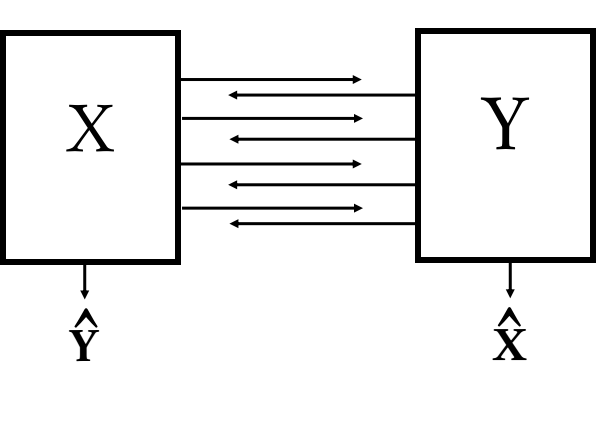
\includegraphics[width=0.4\textwidth]{dataex.png}
  \end{center}
  \caption{The Data-Exchange Problem}
  \label{fig:dataex}
\end{wrapfigure}
A working solution for this problem is r-sync protocol, as described in   \cite{rsync}.The algorithm identifies parts of the source file which are identical to some part of the destination file, and only sends those parts which cannot be matched in this way.Though this protocol is fast and low complexity, it does not exploit the correlation of the data to the best extent possible.In fact, we can view r-sync as an algorithm which uses only one guess, and thus ends up using more communication.\\
In \cite{sw}, David Slepian and Jack Wolf had shown that the optimal solution to this problem is Slepian-Wolf compression. 
\paragraph{Slepian-Wolf Coding Theorem:}states under joint decoding of X and Y a total rate H(X,Y) is sufficient.\\
\begin{wrapfigure}{r}{0.5\textwidth}
  \begin{center}
    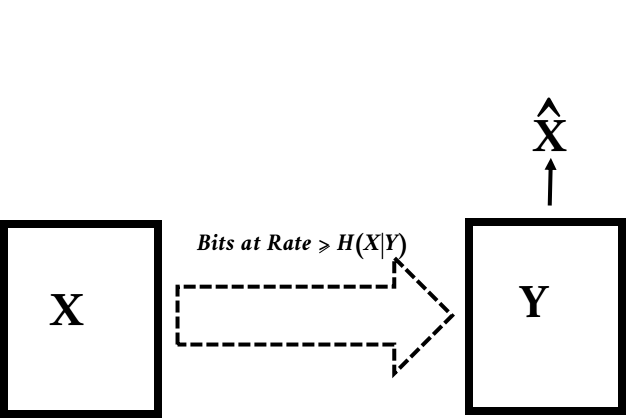
\includegraphics[width=0.4\textwidth]{swcomp.png}
  \end{center}
  \caption{The Slepian-Wolf Compression}
  \label{fig:swcomp}
\end{wrapfigure}
Consider first the problem where X and Y are correlated discrete-alphabet memoryless sources, we have to compress X losslessly, with Y (side information) being known at the decoder and \emph{not} at the encoder. If Y were known at both ends one can compress X at a theoritical rate of $H(X|Y)$. But if Y were known only at decoder the same can be achieved by just knowing $P_{X|Y}$ at encoder without explicit information of Y, this has been depicted in figure\ref{fig:swcomp} \cite{discus}. 
\\\\
A practical implementation of Slepian Wolf compression faces the following difficulties.
\begin{itemize}
\item Search is over an exponential list in decoding.
\item Knowledge of $P_{X|Y}$ is required.
\end{itemize} 

Using structured channel codes as indicated in \cite{discus}, particularly Polar Codes as shown in \cite{pslep}, alongwith \emph{recursive data exchange protocol}  mentioned in \cite{htsw} for Slepian-Wolf compression eases the aforementioned implementation. 

\subsection{Suggested Approach for Solving The Data-Exchange Problem}
In accordance with the above discussion the suggested approach towards solving \emph{the Data-Exchange Problem} may be briefed as follows.
\begin{itemize}
\item{Implement Slepian-Wolf Compression using Polar Codes.}
\item{Achieve universality using \emph{Recursive Data Exchange} protocol (RDE).}
\item{Realise RDE using Rateless Polar Codes with Physical layer Error Detection.}
\end{itemize}

The following sub-sections discuss the artefacts needed for this implementation in brief. Section \ref{propsol}, consolidates and elaborates the proposed scheme. 

\subsection{Interactive Communication for Data Exchange}
The data exchange protocol is based on an interactive version of the Slepian-Wolf protocol where the length of communication is increased in steps until the second party decodes the data of the first. After each transmission second party sends ACK-NACK feedback signal, the protocol stops when ACK is recieved or $l_{max}$ bits have been transmitted \cite{htsw}. Note, this protocol is universal as it does not rely on knowledge of the joint distribution, instead uses an iterative variable length approach to reach rate optimality universally. The decoders suggested in \cite{htsw} are theoritical constructs which use type classes to form a list of guesses for data of other parties and thus has exponential complexity.\\ In \cite{pslep}, Slepian Wolf compression is approached with structered (Polar) codes, in this work we use Rateless Polar Codes to implement RDE with a similar ideology.

\subsection{Brief Introduction to Polar Codes}
\begin{wrapfigure}{r}{0.5\textwidth}
  \begin{center}
    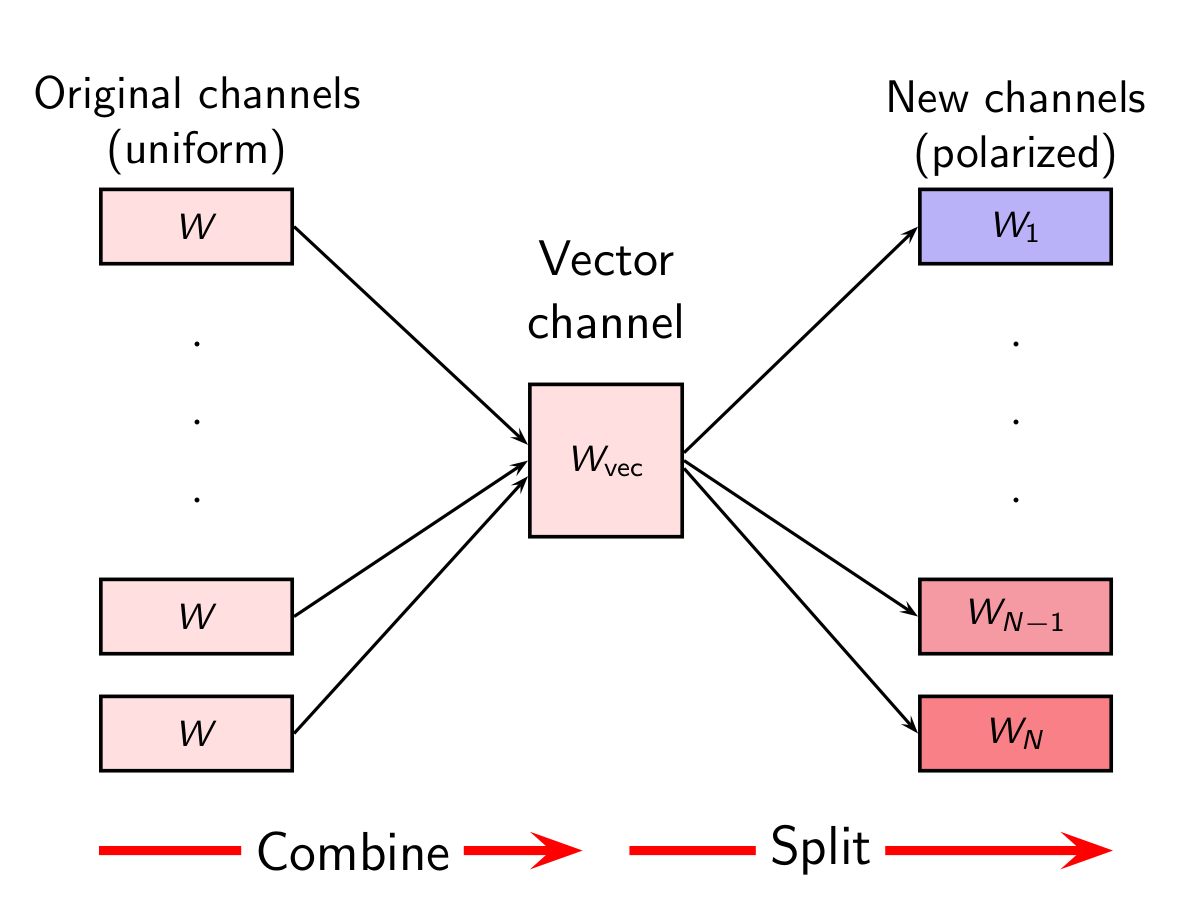
\includegraphics[width=0.4\textwidth]{channelcomb.png}
  \end{center}
  \caption{Channel combining and splitting}
  \label{fig:channelcomb}
\end{wrapfigure}
In 2008, E. Arikan in his paper \cite{arikan} introduced Polar Codes, which provably achieves capacity on symmetric channels. Polar Codes rely on the phenomenon of channel polarization which can be described as follows.
\begin{wrapfigure}{r}{0.5\textwidth}
  \begin{center}
    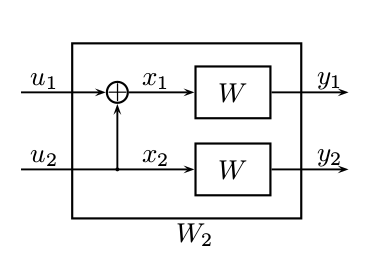
\includegraphics[width=0.4\textwidth]{arikanfly.png}
  \end{center}
  \caption{Arikan transformation butterfly}
  \label{fig:arikanfly}
\end{wrapfigure}
\paragraph{channel polarization}is an operation by which one manufactures out of N independent copies of a given B-DMC W, a second set of N channels $\{W^{(i)}_N : 1 \leq i \leq N \}$ that show a polarization effect in the sense that, as N becomes large,the symmetric capacity terms $I(W^{(i)}_N )$ tend towards 0 or 1,for all but a vanishing fraction of indices i. Alternatively, Bhattacharya parameter $Z(W^{(i)}_N)$ tend to 1 or 0 respectively. 

This operation consists of a channel combining and a channel splitting phase, as shown in figure \ref{fig:channelcomb}. The channel transformation for two independent channels is shown in \ref{fig:arikanfly},this is used recursively. \\The encoding process sends data on transformed channels with $Z(W^{(i)}_N)=0$  (\emph{good channels}) and treats the channels with $Z(W^{(i)}_N)=0$ as \emph{bad or frozen}, thus sending no useful data on them. This scheme of error control coding with polar codes is illustrated in figure \ref{fig:pchscheme}.
\begin{figure}[h]
 \begin{center}
    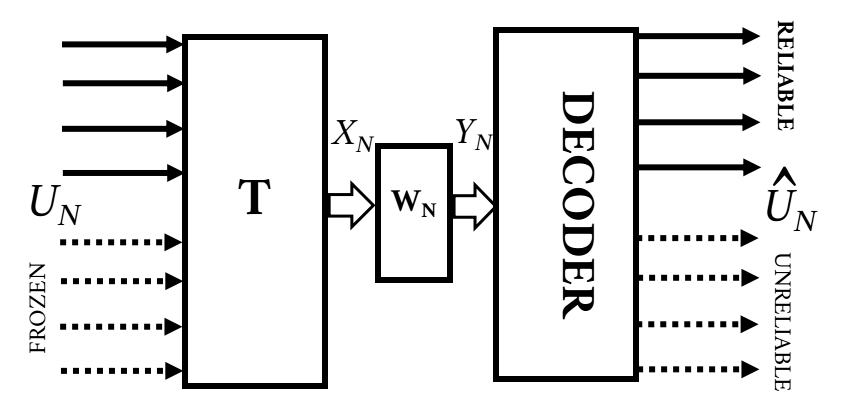
\includegraphics[width=0.6\textwidth]{pchscheme.png}
  \end{center}
  \caption{Polar Coding}
  \label{fig:pchscheme}
\end{figure}\\
In figure \ref{fig:pchscheme}, $U_N$ is a uniform message vector, $T$ is a linear transform equivalent to the butterfly in figure \ref{fig:arikanfly} for a block length of N. It is useful to note here that $T=T^{-1}$.
\begin{figure}[h]
  \begin{center}
    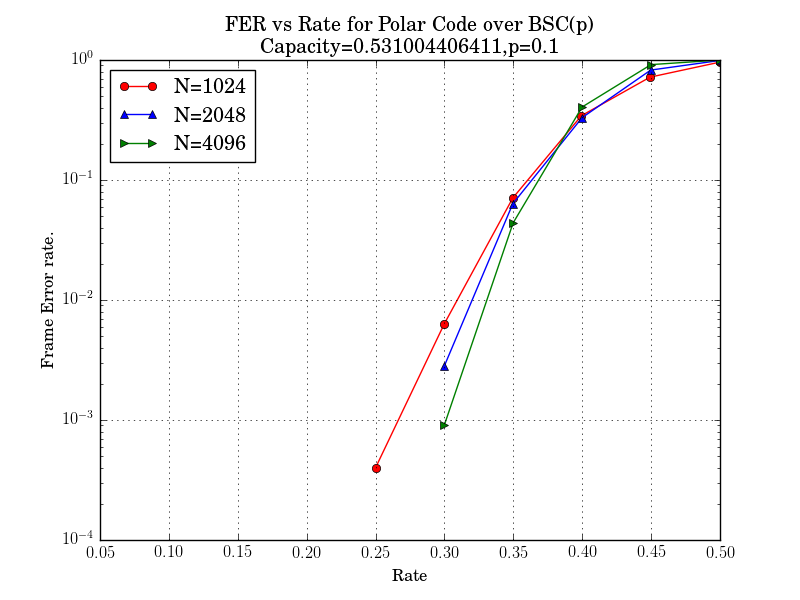
\includegraphics[width=0.6\textwidth]{fer.png}
  \end{center}
  \caption{FER vs Rate for Polar Coding with SC}
  \label{fig:fer}
\end{figure}\\
For our purpose, we shall be using Succesive Cancellation (SC) decoding. Each independent channel will considered as BSC(p). The Polar Code construction indicated in \cite{zhang} has been employed for simplicity. A performance analysis of implementation of the scheme in figure \ref{fig:pchscheme} is presented in figure \ref{fig:fer}    

\subsection{Implementation of SW Compression using Polar Codes}
\begin{figure}[h]
 \begin{center}
    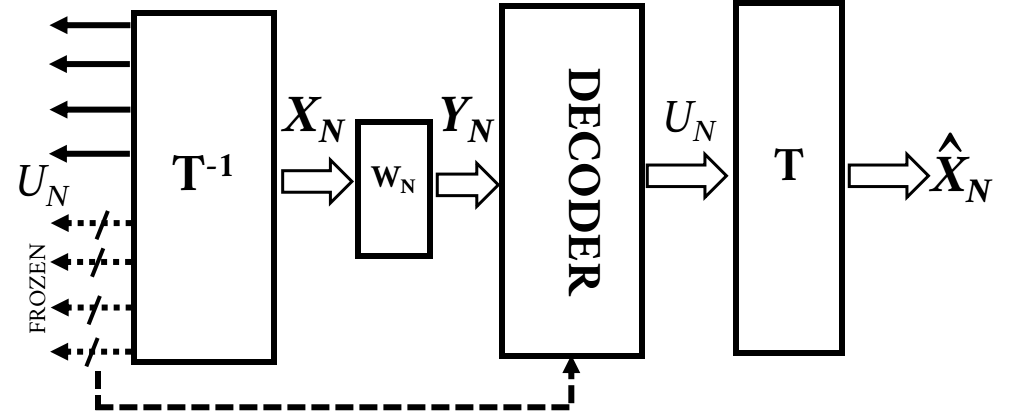
\includegraphics[width=0.6\textwidth]{pswscheme.png}
  \end{center}
  \caption{Polar Coding for SW Compression}
  \label{fig:pswscheme}
\end{figure}
In \cite{discus}, the use of structured codes for Slepian-Wolf compression has been discussed.Further, in \cite{pslep} a specific scheme using Polar Codes has been illustrated, as shown in figure \ref{fig:pswscheme}.\\
Consider the setting where $X_N$ and $Y_N$ are uniform. $Y_N$ is a corrupted version of $X_N$ by a BSC(p). The bits that are to be sent for estimation of $X_N$ from $Y_N$ are the frozen bits in $U_N$. In other words applying $T^{-1}$ to $X_N$ and choosing the bits at frozen positions (the syndrome) essentially describes the compression operation. These bits are communicated error free to the SC-Decoder. On applying $T$ to the output of SC-decoder the estimate $\hat{X}_N$ is received. It is to be noted here that in general the frozen positions are set to 0 in channel coding but in Slepian-Wolf compression they are non-zero by the nature of the scheme. Performance analysis of this scheme is presented in figure \ref{fig:swfer}.
\begin{figure}[h]
 \begin{center}
    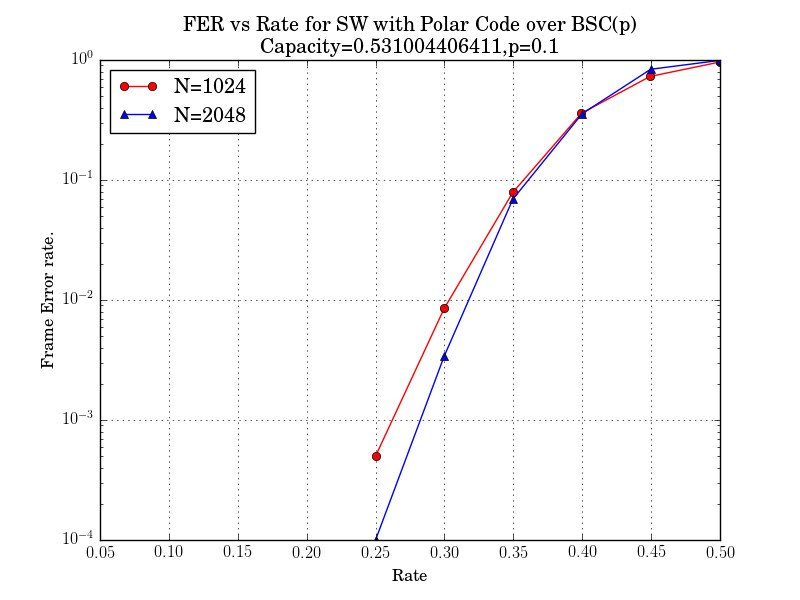
\includegraphics[width=0.6\textwidth]{swfer.png}
  \end{center}
  \caption{FER vs Rate for SW with Polar Code}
  \label{fig:swfer}
\end{figure}\\
Intuitively, a method to generate the syndrome incrementally will lead us to an implementation of RDE. Rateless Polar Codes will be instrumental to accomplish this.

\subsection{Rateless Polar codes}
\paragraph{Rateless code:}A rateless coding scheme transmits incrementally more and more coded bits over an unknown channel until all the information bits are decoded reliably by the receiver. A fixed rate code is designed for a specific channel. In contrast, a rateless code is designed for a set of channels and judged for its performance for the entire set (the compound channel). In general a rateless code design is based on hybrid-ARQ techniques and uses code puncturing. \\For Polar Codes, puncturing is not straightforward. Hybrid-ARQ schemes and puncturing of Polar Codes has been proposed and compared in \cite{harqtav},\cite{harqcheng},and \cite{harqchen}.\\ In \cite{chen}, the authors have proposed a provably capacity achieving rateless coding scheme based on Polar Codes. This scheme is useful for broad class of channels as long as they are ordered by degradation.\footnote{using construction methods in \cite{wang},\cite{mondelli} this method can be extended to a broader class of \emph{less noisy} ordered channels}. The scheme stems from the inherent nesting property and degradedness of Polar codes, this makes puncturing a relatively simple affair. 

\subsubsection{Degradedness and Nesting Property}
\begin{wrapfigure}{r}{0.5\textwidth}
  \begin{center}
    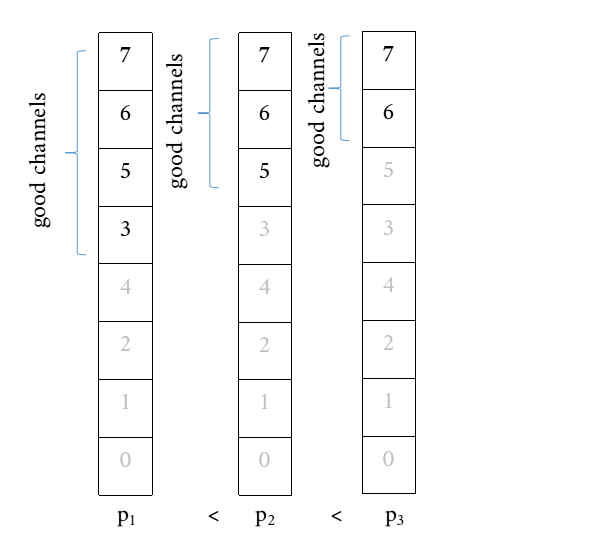
\includegraphics[width=0.5\textwidth]{relorder.png}
  \end{center}
  \caption{Nesting in BSC(p) channels}
  \label{fig:relorder}
\end{wrapfigure}
\paragraph{Degraded channels:}A symmetric binary input channel $W_2$ is said to be degraded with respect to a channel $W_1$ if there exists random variables X,Y,Z such that X\---Y\---Z forms a Markov chain and $W_1=P_{Y|X} , W_2=P_{Z|X}$. By Data Processing Inequality it is evident that the capacity of $W_2$ is lesser than that of $W_1$. This is denoted by $W_2 \preceq W_1$. For example, $BSC(p_1) \preceq BSC(p_2)$ if $p_1 \geq p_2$.
\paragraph{Nesting Property:}Polarization suggests that $W_2 \preceq W_1$ will reflect as lesser number of \emph{good channels} for $W_2$. As the polarization operation preserves degradedness, the good bit indices of $W_2$ must be a subset of the good bit indices of $W_1$. This is Nesting Property. This leads to a \emph{reliability ordering} of the channels, such that a more reliable channel is always noiseless if a less reliable channel is noiseless regardless of the underlying channel.
\subsubsection{Incremental freezing}
These Rateless Polar Coding coding scheme described in \cite{chen} can be described as follows.
Given the reliability ordering, a rateless scheme can be designed as follows. The initial transmission can be done using a high rate polar code with many information bits less frozen bits. If this transmission cannot be decoded\footnote{Decodability is checked by CRC in higher layers.} then among the informations bits sent, the ones on comparatively lesser reliable channels are retransmitted. By decoding these bits from future transmissions they effectively become frozen, allowing the rest of the information bits sent on the first transmission to be decoded. Thus, this scheme can be called \emph{incremental freezing}, as future transmissions successively freeaze more and more bits sent in earlier transmission.
\begin{figure}[h]
 \begin{center}
    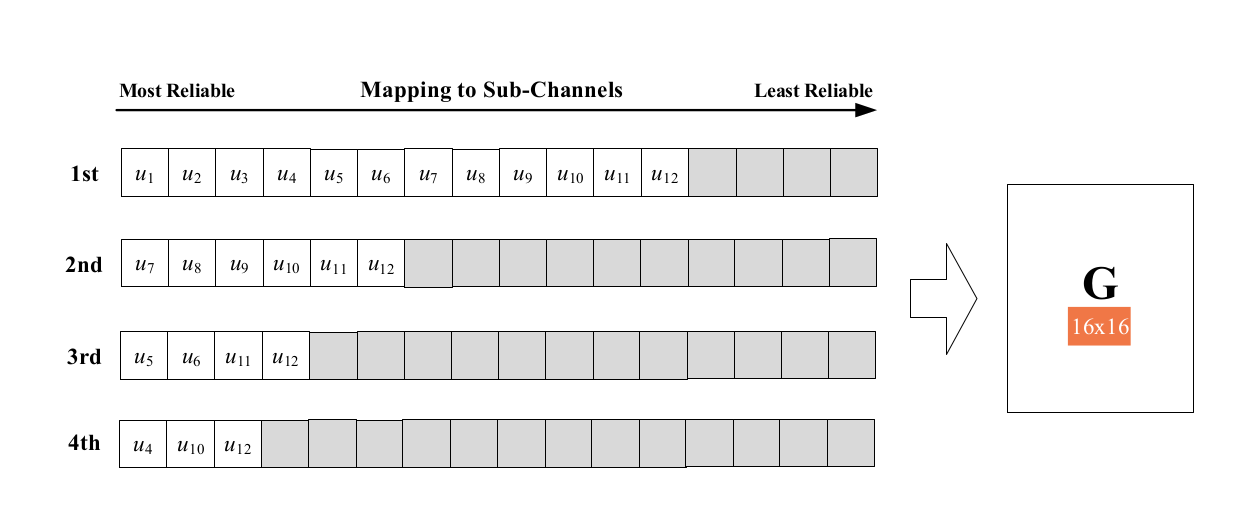
\includegraphics[width=1\textwidth]{if.png}
  \end{center}
  \caption{Incremental freezing for N=16, K=12 and 4 iterations}
  \label{fig:if}
\end{figure}  
\\Figure \ref{fig:if} illustrates the scheme for a set of channels with rates $\{ R=12/16, R_1= R/2,R_2= R/3,R_3= R/4\}$. Here $u_i$ are the message bits. Note that with the $4^th$ transmission  $u_4$ to $u_{12}$ has been incrementally frozen. This scheme is capacity achieving in the sense that no rate has been wasted, the final rate achieved is, $$R^*= \frac{12}{16x4}=\frac{3}{16}=R_3 $$. In case the real channel has capacity $ \geq R_3$ the scheme stops at appropriate iteration to achieve that capacity.\\
Though this scheme is not truly rateless as it can achieve only R, R/2, R/3,...rather than a set of arbitrary rates , adding new information bits in future transmissions allow us to rectify this. In similar fashion this can be extended to parallel channels.\\
It is useful to note taht a certain number of channels in this scheme is "\emph{always available}" guaranteeing a certain rate in each transmission. A specific application of this will be discussed in section \ref{future}.
\subsubsection*{H-ARQ for Polar codes}
\subsubsection*{Rate Compatible Polar Codes}
\subsubsection*{H-ARQ schemes}
\subsubsection*{Reliability Based H-ARQ}


%----------------------------------------------------------------------------------------
%	PROPOSED SOLUTION
%----------------------------------------------------------------------------------------
\newpage
\section{Proposed implementation of Recursive Data Exchange} \label{propsol}

Let $\mathcal{C}$ denote an $(N, K)$ proper binary linear code with length $N$ ,dimension $K$ ,minimum distance ($d_{min}$) atleast 2,and rate defined by $r \triangleq K/N$. We assume that a random codeword is chosen uniformly from this code and transmitted over a memoryless Binary Erasure Channel (BEC).A BEC with erasure probability $p$ is denoted by BEC($p$),or BEC($\underline{p}$) in case the erasure probability is different for each bit where $\underline{p} = (p_1 , \ldots , p_n)$ and
$p_i$ indicates the erasure probability for bit $i$.
The input and output alphabets of the BEC are denoted by $\mathcal{X} = \{0, 1\}$ and $\mathcal{Y} = \{0, 1, e\}$, respectively. Let $\underline{X} = (X_1 , \ldots , X_N) \in \mathcal{X}_N$ be a uniform random codeword and
$\underline{Y} = (Y_1 , \ldots, Y_N) \in \mathcal{Y}_N$ be the received sequence obtained by transmitting $\underline{X}$ through a BEC($p$).For a vector $a = (a_1 , a_2 , \ldots , a_N)$, the shorthand $\underline{a}_{\sim i}$ denotes
$(a_1 , \ldots , a_{i-1} , a_{i+1}, \ldots , a_N)$.
Let $\underline{a}$,$\underline{b}$ denote the indicator vectors of the sets $A \subseteq [N]$,$B \subseteq [N]$.We say that $A$ \emph{covers} $B$ if $B \subseteq A$, equivalently  $\underline{a}\leq\underline{b}$.For linear codes and erasure channels, it is possible to recover the transmitted codeword if and only if the erasure
pattern does not cover any codeword.Similarly,
it is possible to recover bit $i$ if and only if the erasure
pattern does not cover any codeword where bit $i$ is non-zero.


\subsection{Adaptation of Rateless Polar Codes for RDE} 
\paragraph*{Bit error probability:}Let $D_i : \mathcal{Y}^N \to \mathcal{X} \cup \{e\}$ denote the bit-MAP decoder for bit $i$ of $\mathcal{C}$. For a received sequence $\underline{Y}$ , if $X_i$ can be recovered uniquely, then $D_i(\underline{Y}) = X_i$. Otherwise, $D_i$ declares an erasure and returns $e$. Let the erasure probability for bit $i \in [N]$ be $$P_{b,i} \triangleq \mathbb{P}[D_i(\underline{Y}) \neq X_i].$$ and the average bit erasure probability be $$P_b \triangleq \frac{1}{N}\sum_{i=1}^N P_{b,i}.$$

Whenever bit $i$ can be recovered from a received sequence $\underline{Y}=\underline{y}$, $H(X_i | \underline{Y}=\underline{y}) = 0$. Otherwise, the uniform codeword assumption implies that the posterior marginal of bit $i$ given the observations is $\mathbb{P}(X_i = x|\underline{Y}=\underline{y}) = 1/2$ and $H(X_i |\underline{Y}=\underline{y}) = 1$. This immediately implies that $$P_{b,i} = H(X_i|\underline{Y})$$ and, $$P_b = \frac{1}{N}\sum_{i=1}^N  H(X_i|\underline{Y}).$$

\subsection{PHY-Layer error Detection} The vector EXIT function associated with bit $i$ of the (uniformly randomly chosen) codeword is $$h_i(\underline{p})\triangleq H(X_i | \underline{Y}_{\sim i}(\underline{p}_{\sim i})).$$ The average vector EXIT function is defined by $$h(\underline{p}) \triangleq \frac{1}{N}\sum_{i=1}^N h_i(\underline{p}).$$ Scalar EXIT functions are defined by choosing $\underline{p}=(p,p,\ldots,p)$.
\begin{align*}
H(X_i|\underline{Y}) &= \mathbb{P}(Y_i=e)H(X_i|\underline{Y}_{\sim i}, Y_i=e) + \mathbb{P}(X_i=Y_i)H(X_i|\underline{Y}_{\sim i}, Y_i=X_i)\\
&= \mathbb{P}(Y_i=e)H(X_i|\underline{Y}_{\sim i}).
\end{align*}
Therefore, $$P_{b,i}(p) = ph_i(p)$$ and $$P_b(p) = ph(p).$$
\begin{proposition}
The MAP EXIT function for the $i$th bit satisfies $h_i(p)=
\frac{\partial H(\underline{X}/\underline{Y}(\underline{p}))}{\partial p_i} $
\begin{proof}
\begin{align*}
H(\underline{X}/\underline{Y}(\underline{p})) &= H(X_i/\underline{Y}(\underline{p}))+H(X_{\sim i}/X_i,\underline{Y}(\underline{p})\\
&=H(X_i/\underline{Y}(\underline{p}))+H(X_{\sim i}/X_i,Y_{\sim i})  \text{ ,by memorylessness}\\
&=p_ih_i(p)+H(X_{\sim i}/X_i,Y_{\sim i}) 
\end{align*}
We note the second term is independent of $p_{i}$,the proposition follows on differentiation.
\end{proof}
\label{propn1}
\end{proposition}
\paragraph{Indirect Recovery} Consider a code $\mathcal{C}$ and the \emph{indirect recovery} of $X_i$ from the subvector $\underline{Y}_{\sim i}$ (i.e., the bit-MAP decoding of $Y_i$ from $\underline{Y}$ when $Y_i=e$). For $i \in [N]$, the set of erasure patterns that prevent indirect recovery of $X_i$ under bit-MAP decoding is given by 
\begin{definition}
$\Omega_i \triangleq \{A \subseteq [N]\backslash\{i\} : \exists B \subseteq [N]\backslash\{i\}, B \cup \{i\} \in \mathcal{C}, B \subseteq A\}$.
\label{defn2}
\end{definition}
For distinct $i,j \in [N]$, the set of erasure patterns where the $j$-th bit is \emph{pivotal} for the indirect recovery of $X_i$ is given by 
\begin{definition}
$\partial_j\Omega_i \triangleq \{A \subseteq [N]\backslash\{i\}: A\backslash \{j\} \notin \Omega_i, A \cup \{j\} \in \Omega_i \}$
\end{definition}
These are the erasure patterns where $X_i$ can be recovered from $\underline{Y}_{\sim i}$ if and only if $Y_j \neq e$.Note $\partial_j\Omega_i$ includes patterns from both $\Omega_i$ and $\Omega_i^c$.
\begin{proposition}
\label{propn4}
For a code $\mathcal{C}$ and transmission over a BEC, we have the following properties for the EXIT functions.
\begin{enumerate}
\item[(a)] The EXIT function associated with bit $i$ satisfies $$h_i(p) = \mu_{p}(\Omega_i)= \sum_{A \in \Omega_i} p^{|A|}(1-p)^{N-1-|A|}.$$
\item[(b)] For $j \in [N]\backslash\{i\}$, the partial derivative satisfies $$\frac{\partial h_i(\underline{p})}{\partial p_j}\Bigg|_{\underline{p}=(p,p,\ldots,p)} =\mu_{p}(\partial_j\Omega_i)= \sum_{A \in \partial_j\Omega_i} p^{|A|}(1-p)^{N-1-|A|}.$$
\item[(c)]The average EXIT function satisfies the \emph{area theorem} $$\int_0^1 h(p)dp = \frac{K}{N}.$$
\end{enumerate}
Where $\mu_{p}(\Omega)$ is the measure of the set of erasure patterns $\Omega$.
Here (a) and (b) follow from definition of conditional entropy and the fact that $H(X_i/\underline{Y}_{\sim i}=\underline{y}_{\sim i})=1$ when $A \cup \{i\}$ covers some codeword and decoding fails, and $0$ otherwise.(c) is a direct consequence of proposition \ref{propn1}
\end{proposition}
From the above discussion it is clear that the measure of the set $\Omega_i$ is equal to the probability of error for bit i , which in turn is equal to the ith EXIT function due to the uniform input assumption.

\subsubsection{The Error Detection Test } Let $S_N$ be the symmetric group on $N$ elements. The permutation group of a code is defined as the subgroup of $S_N$ whose group action on the bit ordering preserves the set of codewords.\\

\begin{definition}The permutation group $\mathcal{G}$ of a code $\mathcal{C}$ is defined to be $$\mathcal{G} = \{\pi \in S_N : \pi(A) \in \mathcal{C} \text{ for all } A \in \mathcal{C}\}.$$
\end{definition}

\begin{definition} - Suppose $\mathcal{G}$ is a permutation group. Then,
\begin{enumerate}
\item[(a)]$\mathcal{G}$ is \emph{transitive} if, for any $i,j \in [N]$, there exists a permutation $\pi \in \mathcal{G}$ such that $\pi(i)=j$, and
\item[(b)] $\mathcal{G}$ is \emph{doubly transitive} if, for any distinct $i,j,k \in [N]$, there exists a $\pi \in \mathcal{G}$ such that $\pi(i)=i$ and $\pi(j)=k$.
\end{enumerate}
\end{definition}

\begin{proposition}\emph{All EXIT functions are equal.}
Suppose the permutation group $\mathcal{G}$ of a code $\mathcal{C}$ is transitive. Then, for any $i \in [N]$, $$h(p) = h_i(p) \text{ for } 0 \le p\le 1.$$
\begin{proof}
claim:if $\mathcal{G}$ is transitive, then so is $\Omega_i$.
As $ A\in\Omega_i$,by definition\ref{defn2} $\exists B ,s.t.,B\cup\{i\} \in \mathcal{C}$, but by transitivity of $\mathcal{G}$, $\pi(B\cup\{i\}) \in \mathcal{C}$.Observe,$\pi(B\cup\{i\})=\pi(B)\cup\pi(\{i\})=\pi(B)\cup j$.Since $\pi(B) \subseteq \pi(A)$,it follows $\pi(A) \in \Omega_j$ .This indicates a bijection between $\Omega_i$ and $\Omega_j$,i.e,$|\Omega_i|=|\Omega_j|$.Moreover since, $ |A| =|\pi(A)|,$ propostion follows from proposition\ref{propn4} (a)
\end{proof}
\label{propn07}
\end{proposition}


\begin{proposition}
Suppose the permutation group $\mathcal{G}$ of a code $\mathcal{C}$ is doubly transitive. Then, for distinct $i,j,k \in [N]$, and any $0 \le p \le 1$, $$\frac{\partial h_i(\underline{p})}{\partial p_j'}\Bigg|_{\underline{p}=(p,p,\ldots,p)} = \frac{\partial h_i(\underline{p})}{\partial p_k'}\Bigg|_{\underline{p}=(p,p,\ldots,p)}.$$
\begin{proof}
Similar to the proof of proposition 7.Intuitively we expect that once we permute the locations , the bits which were pivotal must continue to remain so.Otherwise we could have decoded the concerned bit using simple permutations.
\end{proof}
\label{propn8}
\end{proposition}
\paragraph*{Summary of properties of EXIT function.}
\begin{description}
\item[1] $h_i(p)$ captures the bit error probability of MAP decoder.
\item[2] $h_i(p)$ is measure of $\Omega_i$.
\item[3] All EXIT functions are equal to average EXIT function h(p).
\item[4] $h_i(p)$ is strictly increasing and invertible.(follows from proposition \ref{propn4} (b))
\item[5] The area under the h vs p curve is the rate( by \emph{Area Theorem}).
\end{description}
We may notice here, that is $A\in\Omega_i$, it is a bit erasure pattern that causes error at position i, then $B\supset A$ will surely cause errors, and $B\in\Omega_i$.Thus $\Omega_i$ is monotone.Proving $\Omega_i $ is symmetric and has a sharp threshold at $p=1-r$, will establish that 2-transitive codes achieve Capacity.We will formalize this in the following subsections.

\subsection{Proposed tests}
\begin{definition}
Suppose $\{\mathcal{C}_n\}$ is a sequence of codes with rates $\{r_n\}$ where $r_n \to r$ for $r \in (0,1)$.
a) $\{\mathcal{C}_n\}$ is said to be \emph{capacity achieving} on the BEC under bit-MAP decoding, if for any $p \in [0, 1-r)$, the average bit-erasure probabilities satisfy $$\lim_{n \to \infty} P_b^{(n)}(p) = 0.$$

\end{definition}
\label{def10}

%\begin{figure}[h]
%\centering 
%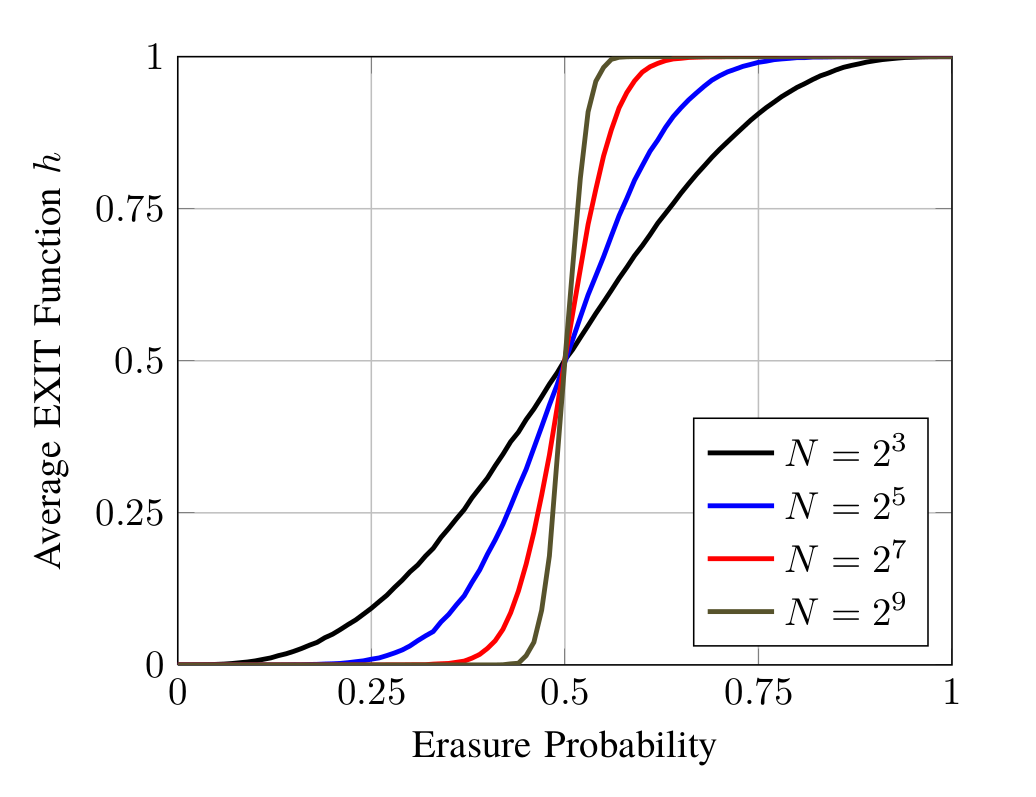
\includegraphics[width=0.75\columnwidth]{exitfun} 
%\caption[]{The average EXIT function of the rate-$1/2$ Reed-Muller code with blocklength $N$.} % The text in the square bracket is the caption for the list of figures while the text in the curly brackets is the figure caption
%\label{fig:exit} 
%\end{figure}

The following theorem bridges capacity achieving codes, average EXIT functions, and the sharp transition framework that allows us to show that the transition width of certain functions goes to $0$. The average EXIT functions of some rate-$1/2$ Reed-Muller codes are shown in Figure~\ref{fig:exit}. Observe that as the blocklength increases, the transition width of the average EXIT function decreases. According to the following proposition, if this width converges to $0$, then Reed-Muller codes achieve capacity on the BEC under bit-MAP decoding.
\begin{proposition}
Let $\{\mathcal{C}_n\}$ be a seq. of codes with rates $\{r_n\}$, $r_n \to r$ for $r \in (0,1)$. The following are equivalent -
\begin{enumerate}
\item[S1:] $\{\mathcal{C}_n\}$ is capacity achieving on the BEC under bit-MAP decoding.
\item[S2:] The sequence of average EXIT functions satisfies
\[
    \lim_{n \to \infty} h^{(n)}(p)=\left\{
                \begin{array}{ll}
                  0 \text{ if } 0 \le p < 1-r\\
                  1 \text{ if } 1-r < p \le 1.\\
                \end{array}
              \right.
  \]
\item[S3:] For any $0 < \epsilon \le 1/2$, $$\lim_{n \to \infty} p_{1-\epsilon}^{(n)} - p_{\epsilon}^{(n)} = 0.$$
\end{enumerate}
\label{propn11}
\end{proposition}
\emph{where $h^{(n)}(p_{\epsilon}^{(n)})=\epsilon$.}\\
In short $S1\Rightarrow S2$, due to close relationship between bit error probability and average EXIT function pointed out in propostion \ref{propn4} .$S2\Rightarrow S3$,and $S3\Rightarrow S1$ by area theorem.Hence, proving S3 suffices to complete the proof.
\subsection{Performance Evaluation}

%--------------------------------------------------------------------------
% CONCLUSION AND FUTURE WORK
%--------------------------------------------------------------------------
\newpage
\section{Conclusion and Future work}\label{future}
proposed scheme
shortpacket
implementation
\begin{definition}
We can redefine $\Omega_i$ as a set of indicator vectors of $A$.Let,
\[
    [\phi_i(A)]_l=\left\{
                \begin{array}{ll}
                  \mathbf{1}_A(l) \text{ if } l < i\\
                  \mathbf{1}_A(l+1) \text{ if } l \ge i.\\
                \end{array}
              \right.
  \]
\begin{align*}
\Omega_i' &\triangleq \{\phi_i(A) \in \{0,1\}^{N-1} : A \in \Omega_i\}\\
\partial_j\Omega_i' &\triangleq \{\phi_i(A) \in \{0,1\}^{N-1}: A \in \partial_j\Omega_i\}.\\& =\{\underline{x} \in \{0,1\}^{N-1} | \mathbb{1}_{\Omega_i}(\underline{x}) \neq  \mathbb{1}_{\Omega_i}(\underline{x}^{(j)})\}
\end{align*}
\label{defn13}
\end{definition}
Here the last equality follows from definition of $\partial_j\Omega_i$.\\
Consider the space $\{0,1\}^M$ ,we can redefine measure $\mu_p$ such that $$\mu_p(\Omega) = \sum_{\underline{x} \in \Omega} p^{|\underline{x}|}(1-p)^{M-|\underline{x}|}, \text{ for }\Omega \subseteq \{0,1\}^M,$$ where the weight $|\underline{x}| = x_1 + x_2 + \ldots + x_M$ is the number of $1$'s in $\underline{x}$. 
\begin{definition}
For a monotone set $\Omega$.The influence of bit $j \in [N]$,is defined by,
$$I_j^{(p)}(\Omega)\triangleq \mu_p(\partial_j\Omega)$$
The total influence in defined by,
$$I^{(p)}\triangleq \sum^N_{j=1}I_j^{(p)}.$$
\label{defn15}
\end{definition}
Using proposition~\ref{propn4}(a) and proposition 7, we have, 
$$h(p)=h_i(p)=\mu_p(\Omega_i')$$
Further,from proposition~\ref{propn4}(b), we get,
$$I_j^{p}(\Omega_i')=\mu_p(\partial_j\Omega_i') = \frac{\partial h_i(\underline{p})}{\partial p_j'}\Bigg|_{\underline{p}=(p,p,\ldots,p)}$$
where $j'$ is given by 
\[
    j'=\left\{
                \begin{array}{ll}
                  j \text{ if } j < i\\
                  j+1 \text{ if } j \ge i.\\
                \end{array}
              \right.
  \]
Since $\mathcal{G}$ is doubly transitive, from propostion~\ref{propn8}, $$I_j^{p}(\Omega_i') = I_k^{p}(\Omega_i') \text{ for all } j,k \in [N-1].$$
Hence,$\Omega_i$ is a \emph{symmetric monotone set.}

The following theorem could be seen as a consequence of the result by Talagrand~\cite{talagrand}.
\begin{theorem}
Let $\Omega$ be a monotone set and suppose that, for all $0 \le p \le 1$, the influences of all bits are equal $I_1^{(p)}(\Omega) = \ldots = I_M^{(p)}(\Omega)$. Then, for any $0 < \epsilon \le 1/2$, $$p_{1-\epsilon} - p_\epsilon \le \frac{2 \log \frac{1-\epsilon}{\epsilon}}{C\log (N-1)},$$ where $p_t = \inf\{p \in [0,1] : \mu_p (\Omega) \ge t\}$ is well defined because $\mu_p(\Omega)$ is strictly increasing in $p$ with $\mu_0(\Omega) = 0$ and $\mu_1(\Omega)=1$.
\label{thm19}
\end{theorem}
\begin{proof}
Using Russo's lemma~\cite{russo}.
\end{proof}
We see that $\Omega_i$ satisfies the conditions of Theorem~\ref{thm19}.
Hence,\\$$\lim_{n \to \infty} (p_{1-\epsilon} - p_\epsilon) = 0.$$
Further , using proposition~\ref{propn11}, we state,\emph{\\$\{\mathcal{C}_n\}$ is capacity achieving on the BEC under bit-MAP decoding.}


%----------------------------------------------------------------------------------------
%	BIBLIOGRAPHY
%----------------------------------------------------------------------------------------
\newpage
\renewcommand{\refname}{\spacedlowsmallcaps{References}} % For modifying the bibliography heading

\bibliographystyle{unsrt}

\bibliography{polarmid.bib} % The file containing the bibliography

%----------------------------------------------------------------------------------------

\end{document}